\section{Extended Experimental Results}
\label{sec:extended-results}

\subsection{Main Results: ImageNet-100 (10-class)}
\label{sec:results-10cls}

\Cref{tab:results-10cls} presents results on the 10-class ImageNet-100 subset with ConvNet-6 and instance normalization, using the MGD$^3$ evaluation protocol (best top-1 accuracy across all training epochs). The unguided baseline achieves $49.73 \pm 1.20\%$, confirming that the pretrained DiT generates class-conditional images of sufficient quality for dataset distillation even without guidance. Fixed guidance at $\lambda = 0.05$ yields $49.00 \pm 0.71\%$, a $-0.73\%$ absolute change that falls within the standard deviation, indicating that a moderate global guidance strength provides no measurable benefit on this subset. \cags{} at the matching average guidance range $[0.0, 0.08]$ achieves $49.40 \pm 0.28\%$, which is statistically indistinguishable from unguided ($-0.33\%$ absolute, within one standard deviation). However, \cags{} does improve top-5 accuracy: $84.87 \pm 0.19\%$ vs.\ unguided $83.20 \pm 0.65\%$ ($+1.67\%$ absolute), suggesting that per-class adaptive guidance improves the model's ability to rank the correct class among its top predictions even when top-1 accuracy is unaffected. The neutral top-1 result on 10-class IPC=10 contrasts sharply with the strong gains observed on the 100-class subset (\Cref{sec:results-100cls}), and we attribute this to the limited class complexity variation when only 10 classes are present---a hypothesis we validate in \Cref{tab:ipc-ablation-10cls}.

\begin{table}[t]
\centering
\caption{ImageNet-100 (10-class) results with ConvNet-6, IPC=10, 3 seeds. Best-accuracy tracking per MGD$^3$ protocol. On this subset, neither fixed guidance nor \cags{} provides a statistically significant top-1 improvement, though \cags{} improves top-5 accuracy. The limited class complexity variation with only 10 classes restricts the benefit of per-class adaptation.}
\label{tab:results-10cls}
\begin{tabular}{lcccc}
\toprule
\textbf{Method} & \textbf{Avg. $\lambda$} & \textbf{Top-1 (\%)} & \textbf{Top-5 (\%)} & \textbf{$\Delta$ top-1} \\
\midrule
Unguided & 0.000 & $49.73 \pm 1.20$ & $83.20 \pm 0.65$ & --- \\
Fixed $\lambda = 0.05$ & 0.050 & $49.00 \pm 0.71$ & $83.60 \pm 0.98$ & $-0.73$ \\
\midrule
\cags{} $[0.0, 0.08]$ & $\sim$0.055 & $49.40 \pm 0.28$ & $\mathbf{84.87 \pm 0.19}$ & $-0.33$ \\
\bottomrule
\end{tabular}
\end{table}

\paragraph{IPC ablation reveals boundary conditions.}
\Cref{tab:ipc-ablation-10cls} presents the full IPC ablation on the 10-class subset. At IPC=50, \cags{} achieves $69.87 \pm 1.43\%$ vs.\ unguided $64.73 \pm 0.77\%$ ($+5.13\%$ absolute, $+7.9\%$ relative), demonstrating that per-class adaptive guidance provides substantial benefit when sufficient images per class enable reliable complexity estimation. At IPC=10, as discussed above, \cags{} is neutral. Critically, at IPC=1, \cags{} \emph{degrades} performance to $19.87 \pm 0.90\%$ vs.\ unguided $22.80 \pm 0.16\%$ ($-2.93\%$ absolute, $-12.8\%$ relative). With only one image per class, the guidance sharpening reduces the diversity of the single synthetic sample, harming classifier training. \iast{} partially mitigates this degradation ($21.13 \pm 0.09\%$, $+1.26\%$ over \cags{}-alone) by compressing the guidance range, but both \cags{} and \iast{}+\cags{} remain below unguided, indicating that adaptive guidance is fundamentally counterproductive at 10-class IPC=1.

Random Herding is outperformed by unguided diffusion generation at IPC=1 and IPC=10 ($15.93\%$ vs.\ $22.80\%$ and $40.13\%$ vs.\ $49.73\%$), but slightly exceeds unguided at IPC=50 ($65.47\%$ vs.\ $64.73\%$, $+1.1\%$ relative). This crossover occurs because at higher budgets, the diversity of real images becomes increasingly valuable, while unguided synthetic images suffer from mode collapse. However, \cags{} surpasses Random Herding at IPC=50 by $+4.40\%$ absolute ($69.87\%$ vs.\ $65.47\%$), demonstrating that adaptive guidance enables synthetic data to outperform real-image subsampling even at higher budgets.

\begin{table}[t]
\centering
\caption{IPC ablation on ImageNet-100 (10-class) with ConvNet-6, 3 seeds. Best-accuracy tracking per MGD$^3$ protocol. \cags{} $[0.0, 0.08]$ provides large gains at IPC=50 ($+7.9\%$ relative) but is neutral at IPC=10 and \emph{harmful} at IPC=1 ($-12.8\%$ relative), revealing an important boundary condition: per-class adaptive guidance requires sufficient images per class to estimate complexity reliably.}
\label{tab:ipc-ablation-10cls}
\begin{tabular}{lccc}
\toprule
\textbf{Method} & \textbf{IPC=1} & \textbf{IPC=10} & \textbf{IPC=50} \\
\midrule
Random Herding & $15.93 \pm 0.57$ & $40.13 \pm 0.90$ & $65.47 \pm 0.62$ \\
Unguided & $22.80 \pm 0.16$ & $49.73 \pm 1.20$ & $64.73 \pm 0.77$ \\
Fixed $\lambda = 0.05$ & --- & $49.00 \pm 0.71$ & --- \\
\cags{} $[0.0, 0.08]$ & $19.87 \pm 0.90$ & $49.40 \pm 0.28$ & $\mathbf{69.87 \pm 1.43}$ \\
\iast{}+\cags{} & $21.13 \pm 0.09$ & --- & --- \\
\midrule
$\Delta$ \cags{} vs.\ unguided (rel.) & $-12.8\%$ & $-0.7\%$ & $+7.9\%$ \\
$\Delta$ \iast{}+\cags{} vs.\ unguided (rel.) & $-7.3\%$ & --- & --- \\
\bottomrule
\end{tabular}
\end{table}

\subsection{Module Ablation on 100-class}
\label{sec:module-ablation}

To understand the contribution of each \ags{} module, we evaluate module combinations on the 100-class subset where \cags{} demonstrates the strongest effect (\Cref{tab:module-ablation}). The unguided baseline achieves $22.79 \pm 0.18\%$, and fixed $\lambda = 0.10$ slightly decreases performance to $21.31 \pm 0.42\%$, confirming that fixed guidance is harmful on this subset. \cags{} $[0.0, 0.06]$ alone improves to $25.29 \pm 0.27\%$ ($+10.9\%$ relative). Adding \tags{} (linear schedule) on top of \cags{} yields $22.73 \pm 0.15\%$, which improves over unguided by $-0.06\%$ ($-0.3\%$ relative) but \emph{underperforms} \cags{}-alone by $2.56\%$. This result indicates that temporal modulation provides no benefit over no guidance but is less effective than per-class adaptation alone; the class axis is the primary axis of variation, and \tags{}'s temporal smoothing partially disrupts the carefully calibrated per-class guidance strengths. By design, \iast{} has no effect at IPC=10 (the range scale equals 1.0), so \iast{}+\cags{} is equivalent to \cags{}-alone at this budget.

\begin{table}[t]
\centering
\caption{Module ablation on ImageNet-100 (100-class) with ConvNet-6, IPC=10, 3 seeds. Best-accuracy tracking per MGD$^3$ protocol. \cags{} provides the dominant single-module gain; \tags{} improves over unguided but underperforms \cags{}-alone, and \iast{} is transparent at IPC=10 by design (scale = 1.0).}
\label{tab:module-ablation}
\begin{tabular}{lcc}
\toprule
\textbf{Configuration} & \textbf{Top-1 (\%)} & \textbf{$\Delta$ vs.\ unguided} \\
\midrule
Unguided (MGD$^3$ baseline) & $22.79 \pm 0.18$ & --- \\
Fixed $\lambda = 0.10$ & $21.31 \pm 0.42$ & $-1.48$ \\
\midrule
\cags{} $[0.0, 0.06]$ & $\mathbf{25.29 \pm 0.27}$ & $\mathbf{+2.50}$ \\
\iast{} + \cags{} (IPC=10, equiv.\ to \cags{}) & $25.29 \pm 0.27$ & $+2.50$ \\
\tags{} linear + \cags{} $[0.0, 0.06]$ & $22.73 \pm 0.15$ & $-0.06$ \\
\bottomrule
\end{tabular}
\end{table}

\subsection{IPC Ablation on 100-class}
\label{sec:ipc-ablation}

The 100-class IPC ablation reveals the most nuanced findings of our study (\Cref{tab:ipc-ablation-100cls}). At IPC=1, the unguided baseline achieves $5.79 \pm 0.09\%$, and the optimal two-factor \cags{} improves to $6.51 \pm 0.22\%$ ($+12.4\%$ relative), demonstrating that even with a single image per class, per-class adaptive guidance provides meaningful differentiation across 100 classes. Crucially, \iast{}+\cags{} \emph{reduces} performance to $5.87 \pm 0.07\%$, essentially reverting to unguided levels ($+1.4\%$ relative, within noise). The \iast{} log-scaling factor for IPC=1 is $0.289$, which compresses the guidance range from $[0, 0.06]$ to $[0, 0.017]$. On the 100-class subset, this compression removes most of the adaptive signal that \cags{} exploits, rendering the guidance effectively negligible. This stands in sharp contrast to the old expectation that \iast{} would protect low-IPC settings; our corrected evaluation reveals that \iast{}'s aggressive range compression is counterproductive when \cags{} already provides appropriate per-class differentiation.

The contrast between this result and the 10-class IPC=1 setting (where \cags{} itself \emph{hurts}) reveals an important boundary condition. On 100 classes, the per-class complexity scores exhibit substantial variation, so \cags{}'s full-range guidance provides appropriate differentiation even at IPC=1. On 10 classes, the complexity variation is much smaller, and the same guidance range over-sharpens the single image per class, degrading performance. \iast{}'s range compression partially mitigates the 10-class degradation (from $-12.8\%$ to $-7.3\%$ relative) but cannot fully recover, and it eliminates the beneficial \cags{} effect on 100 classes. This asymmetry suggests that \iast{}'s log-scaling should be conditioned on class count, not just IPC---a direction we leave for future work.

At IPC=10, the optimal two-factor \cags{} improves to $25.70 \pm 0.07\%$ ($+12.8\%$ relative), outperforming the original four-factor configuration ($25.29 \pm 0.27\%$, $+10.9\%$ relative) by $+0.41\%$ absolute with $3.9\times$ lower variance. At IPC=50, the optimal two-factor \cags{} achieves $41.45 \pm 0.11\%$ ($+19.4\%$ relative over unguided $34.71 \pm 0.37\%$), substantially outperforming the original four-factor configuration ($39.85 \pm 0.15\%$, $+14.8\%$ relative) by $+1.60\%$ absolute with $1.4\times$ lower variance. Random Herding at IPC=50 ($34.46 \pm 0.02\%$) is comparable to unguided diffusion generation ($34.71 \pm 0.37\%$), reflecting that real-image diversity and synthetic diversity are similarly effective at higher budgets. However, the optimal \cags{} surpasses Random Herding by $+6.99\%$ absolute ($+20.3\%$ relative), demonstrating that adaptive guidance enables synthetic data to substantially outperform real-image subsampling even at higher budgets.

\begin{table}[t]
\centering
\caption{IPC ablation on ImageNet-100 (100-class) with ConvNet-6, 3 seeds. Best-accuracy tracking per MGD$^3$ protocol. The optimal two-factor \cags{} $(0, 0.5, 0.5, 0)$ provides consistent and substantial gains at all IPC settings ($+12.4\%$ to $+19.4\%$ relative over unguided), outperforming the original four-factor configuration at IPC=10 and IPC=50. \iast{}+\cags{} \emph{hurts} at IPC=1 by compressing the guidance range.}
\label{tab:ipc-ablation-100cls}
\begin{tabular}{lccc}
\toprule
\textbf{Method} & \textbf{IPC=1} & \textbf{IPC=10} & \textbf{IPC=50} \\
\midrule
Random Herding & $3.69 \pm 0.08$ & $14.06 \pm 0.48$ & $34.46 \pm 0.02$ \\
Unguided & $5.79 \pm 0.09$ & $22.79 \pm 0.18$ & $34.71 \pm 0.37$ \\
Fixed $\lambda = 0.10$ & --- & $21.31 \pm 0.42$ & --- \\
\cags{} (4-factor) $[0.0, 0.06]$ & --- & $25.29 \pm 0.27$ & $39.85 \pm 0.15$ \\
\cags{} (2-factor, optimal) & $\mathbf{6.51 \pm 0.22}$ & $\mathbf{25.70 \pm 0.07}$ & $\mathbf{41.45 \pm 0.11}$ \\
\iast{}+\cags{} $[0.0, 0.06]$ & $5.87 \pm 0.07$ & --- & --- \\
\midrule
$\Delta$ \cags{} opt.\ vs.\ unguided (rel.) & --- & $+12.8\%$ & $+19.4\%$ \\
$\Delta$ \iast{}+\cags{} vs.\ unguided (rel.) & $+1.4\%$ & --- & --- \\
\bottomrule
\end{tabular}
\end{table}

\subsection{ImageNette and ImageWoof}
\label{sec:results-nette-woof}

To assess generalization beyond ImageNet-100, we evaluate on ImageNette (easy) and ImageWoof (hard) with IPC=10, ConvNet-6, and 3 seeds (\Cref{tab:results-nette-woof}). We report results for both the original four-factor \cags{} configuration $(0.3, 0.3, 0.2, 0.2)$ and the optimized two-factor configuration $(0, 0.5, 0.5, 0)$ identified by our weight grid search (\Cref{sec:weight-learning}). On ImageNette, both configurations improve over unguided: the original \cags{} achieves $52.64 \pm 0.28\%$ vs.\ unguided $49.99 \pm 0.22\%$ ($+5.3\%$ relative), and the optimal configuration achieves $55.27 \pm 0.68\%$ ($+10.6\%$ relative), confirming that per-class adaptive guidance generalizes to easily classifiable datasets.

On ImageWoof, the two configurations diverge. The original four-factor \cags{} achieves $31.99 \pm 0.46\%$---only marginally above unguided $31.75 \pm 0.06\%$ ($+0.8\%$ relative), a negligible improvement caused by the separability factor's counterproductive near-constant guidance on fine-grained classes. In contrast, the optimal two-factor configuration provides a clearer improvement: it achieves $32.87 \pm 0.29\%$, exceeding unguided by $+1.12\%$ absolute ($+3.5\%$ relative) and the four-factor design by $+0.87\%$ absolute. This is a critical finding: the weight grid search not only improves accuracy on datasets where \cags{} already helps (ImageNette: $+2.63\%$ over original \cags{}), but also \emph{amplifies the benefit} on fine-grained datasets where the original configuration provided minimal gains. The mechanism is clear: eliminating the separability factor ($\delta \to 0$) and mode count ($\alpha \to 0$) removes the near-constant guidance offset that was adding noise on ImageWoof's visually similar classes, allowing the entropy and intra-class variance signals to provide genuinely useful per-class differentiation. This result strengthens the case for the simplified two-factor design and demonstrates that the marginal benefit of the original configuration on fine-grained data was an artifact of suboptimal weight selection, not a fundamental limitation of per-class adaptive guidance.

\begin{table}[t]
\centering
\caption{ImageNette and ImageWoof results with ConvNet-6, IPC=10, 3 seeds. The original four-factor \cags{} $(0.3, 0.3, 0.2, 0.2)$ provides only marginal gains on ImageWoof ($+0.8\%$ relative), but the optimized two-factor configuration $(0, 0.5, 0.5, 0)$ provides clearer improvements ($+3.5\%$ relative), demonstrating that the two-factor design is more effective on fine-grained data.}
\label{tab:results-nette-woof}
\begin{tabular}{llcc}
\toprule
\textbf{Dataset} & \textbf{Method} & \textbf{Top-1 (\%)} & \textbf{Top-5 (\%)} \\
\midrule
ImageNette & Random Herding & $40.82 \pm 0.17$ & $81.38 \pm 0.08$ \\
ImageNette & Unguided & $49.99 \pm 0.22$ & $85.28 \pm 0.21$ \\
ImageNette & \cags{} (4-factor) & $52.64 \pm 0.28$ & $88.37 \pm 0.47$ \\
ImageNette & \cags{} (2-factor, optimal) & $\mathbf{55.27 \pm 0.68}$ & $\mathbf{88.35 \pm 0.35}$ \\
\midrule
ImageWoof & Random Herding & $22.69 \pm 0.16$ & $68.73 \pm 0.16$ \\
ImageWoof & Unguided & $31.75 \pm 0.06$ & $76.33 \pm 0.38$ \\
ImageWoof & \cags{} (4-factor) & $31.99 \pm 0.46$ & $75.69 \pm 0.38$ \\
ImageWoof & \cags{} (2-factor, optimal) & $\mathbf{32.87 \pm 0.29}$ & $\mathbf{76.95 \pm 1.12}$ \\
\bottomrule
\end{tabular}
\end{table}

\subsection{FID Analysis}
\label{sec:fid}

To assess the impact of \cags{} on the fidelity of the generated images, we compute Fr\'echet Inception Distance (FID)~\cite{dufour2026lottery} between synthetic and real validation images (\Cref{tab:fid}). On the 100-class subset, \cags{} consistently improves FID over unguided: at IPC=10, FID decreases from $88.66$ to $85.26$ ($-3.40$), and at IPC=50, from $71.06$ to $59.28$ ($-11.78$). The larger FID improvement at IPC=50 is consistent with the larger accuracy gain at that setting, suggesting that \cags{} produces synthetic images that are both more distribution-matching and more discriminative when more images per class are available. These findings challenge the common assumption that lower FID always corresponds to better downstream utility: \cags{} improves both FID and classification accuracy on the 100-class subset, indicating that the guidance adaptation produces images that are simultaneously more faithful to the real distribution and more discriminative for training.

\begin{table}[t]
\centering
\caption{FID scores (lower is better) for unguided vs.\ \cags{} on the 100-class subset. \cags{} improves FID at both IPC settings, with the larger improvement at IPC=50 consistent with the larger accuracy gain at that setting.}
\label{tab:fid}
\begin{tabular}{llccc}
\toprule
\textbf{Dataset} & \textbf{IPC} & \textbf{Unguided} & \textbf{\cags{}} & \textbf{$\Delta$} \\
\midrule
ImageNet-100 (100-cls) & 10 & $88.66$ & $\mathbf{85.26}$ & $-3.40$ \\
ImageNet-100 (100-cls) & 50 & $71.06$ & $\mathbf{59.28}$ & $-11.78$ \\
\bottomrule
\end{tabular}
\end{table}

\subsection{Class-Level Mechanism Analysis}
\label{sec:class-analysis}

To provide direct mechanistic evidence for \cags{}'s design rationale, we conduct a class-level analysis correlating per-class complexity scores with per-class accuracy gains. We train unguided and \cags{} models on the 100-class subset using the optimal two-factor data (IPC=10, ConvNet-6, 2000 epochs, seed 0) and compute per-class accuracy on the 5{,}000-image validation set. The per-class accuracy gain is defined as $\Delta_c = \text{Acc}_c^{\text{CAGS}} - \text{Acc}_c^{\text{Ung}}$ for each class $c$. The overall top-1 accuracies are $22.50\%$ (unguided) and $26.06\%$ (\cags{}), yielding an overall gain of $+3.56\%$---consistent with the 3-seed main result ($+2.91\%$).

The overall Pearson correlation between the two-factor complexity score $\rho_c$ and per-class gain $\Delta_c$ is $r = 0.138$ ($p = 0.172$), substantially stronger than the near-zero correlation ($r = 0.018$) obtained with the original four-factor weights, but still modest. This weak linear correlation, however, masks a clear non-linear pattern revealed by the quartile analysis (\Cref{tab:quartile-analysis}): the top-half complexity classes (Q3+Q4) exhibit a mean gain of $+5.2\%$, while the bottom-half (Q1+Q2) gain only $+1.9\%$---a $2.8\times$ difference. The highest-complexity quartile (Q4) shows the most favorable ratio of positive to negative gains ($19$ positive, $3$ negative, $3$ zero), confirming that \cags{}'s benefit concentrates on complex classes that require stronger guidance.

Among the individual complexity factors, inter-class separability shows the strongest and statistically significant correlation with per-class gains ($r = 0.205$, $p = 0.041$; Spearman $\rho = 0.285$, $p = 0.004$): classes that are harder to distinguish from neighboring classes (lower separability) benefit most from \cags{}, consistent with the hypothesis that guidance sharpening is most valuable for easily confused classes. Intra-class variance shows a weaker positive trend ($r = 0.114$, $p = 0.259$), and cluster entropy is near-zero ($r = 0.076$, $p = 0.455$). Interestingly, while separability is the strongest per-class predictor of gains, the factor ablation (\Cref{sec:factor-ablation}) reveals that separability alone produces the least per-class guidance variation (std $0.006$) and is the weakest standalone signal. This apparent paradox suggests that separability captures \emph{which classes benefit} from guidance but does not itself generate sufficient per-class variation to drive adaptive guidance; cluster entropy and intra-class variance, which produce wider per-class variation, are more effective as standalone complexity signals. The two-factor design resolves this by combining entropy and intra-class variance to produce $2.3\times$ wider per-class $\lambda$ variation (std $0.0049$ vs.\ $0.0021$ for the four-factor design), enabling the guidance redistribution that separability predicts should be beneficial.

The distribution of per-class gains (\Cref{fig:class-level-mechanism}) further confirms the broad-based nature of \cags{}'s improvement: $62$ of $100$ classes show positive gains, $25$ show negative gains, and $13$ are unchanged, with a mean gain of $+3.6\%$ and median of $+4.0\%$. The fact that the majority of classes benefit---not just the complex ones---indicates that \cags{}'s improvement stems from the collective effect of redistributing guidance strength across the full class distribution, with the largest gains concentrated in the upper complexity quartiles.

\begin{table}[t]
\centering
\caption{Quartile analysis of per-class accuracy gains by two-factor complexity score (100-class, IPC=10, seed 0, 2000 epochs). Higher-complexity quartiles receive stronger guidance ($\lambda$) and exhibit larger mean gains, with Q4 showing the most favorable positive-to-negative ratio ($19{:}3$). The top-half complexity classes (Q3+Q4) gain $2.8\times$ more than the bottom-half (Q1+Q2).}
\label{tab:quartile-analysis}
\begin{tabular}{ccccccc}
\toprule
\textbf{Quartile} & \textbf{Mean $\rho_c$} & \textbf{Mean $\lambda_c$} & \textbf{Ung.\ Acc.} & \textbf{CAGS Acc.} & \textbf{Mean Gain} & \textbf{+/--/=} \\
\midrule
Q1 (low) & $0.470$ & $0.028$ & $0.311$ & $0.335$ & $+0.024$ & $13/8/4$ \\
Q2 & $0.558$ & $0.034$ & $0.225$ & $0.238$ & $+0.014$ & $14/8/3$ \\
Q3 & $0.609$ & $0.037$ & $0.178$ & $0.233$ & $+0.055$ & $16/6/3$ \\
Q4 (high) & $0.680$ & $0.041$ & $0.186$ & $0.236$ & $+0.050$ & $19/3/3$ \\
\bottomrule
\end{tabular}
\end{table}

\begin{figure}[t]
\centering
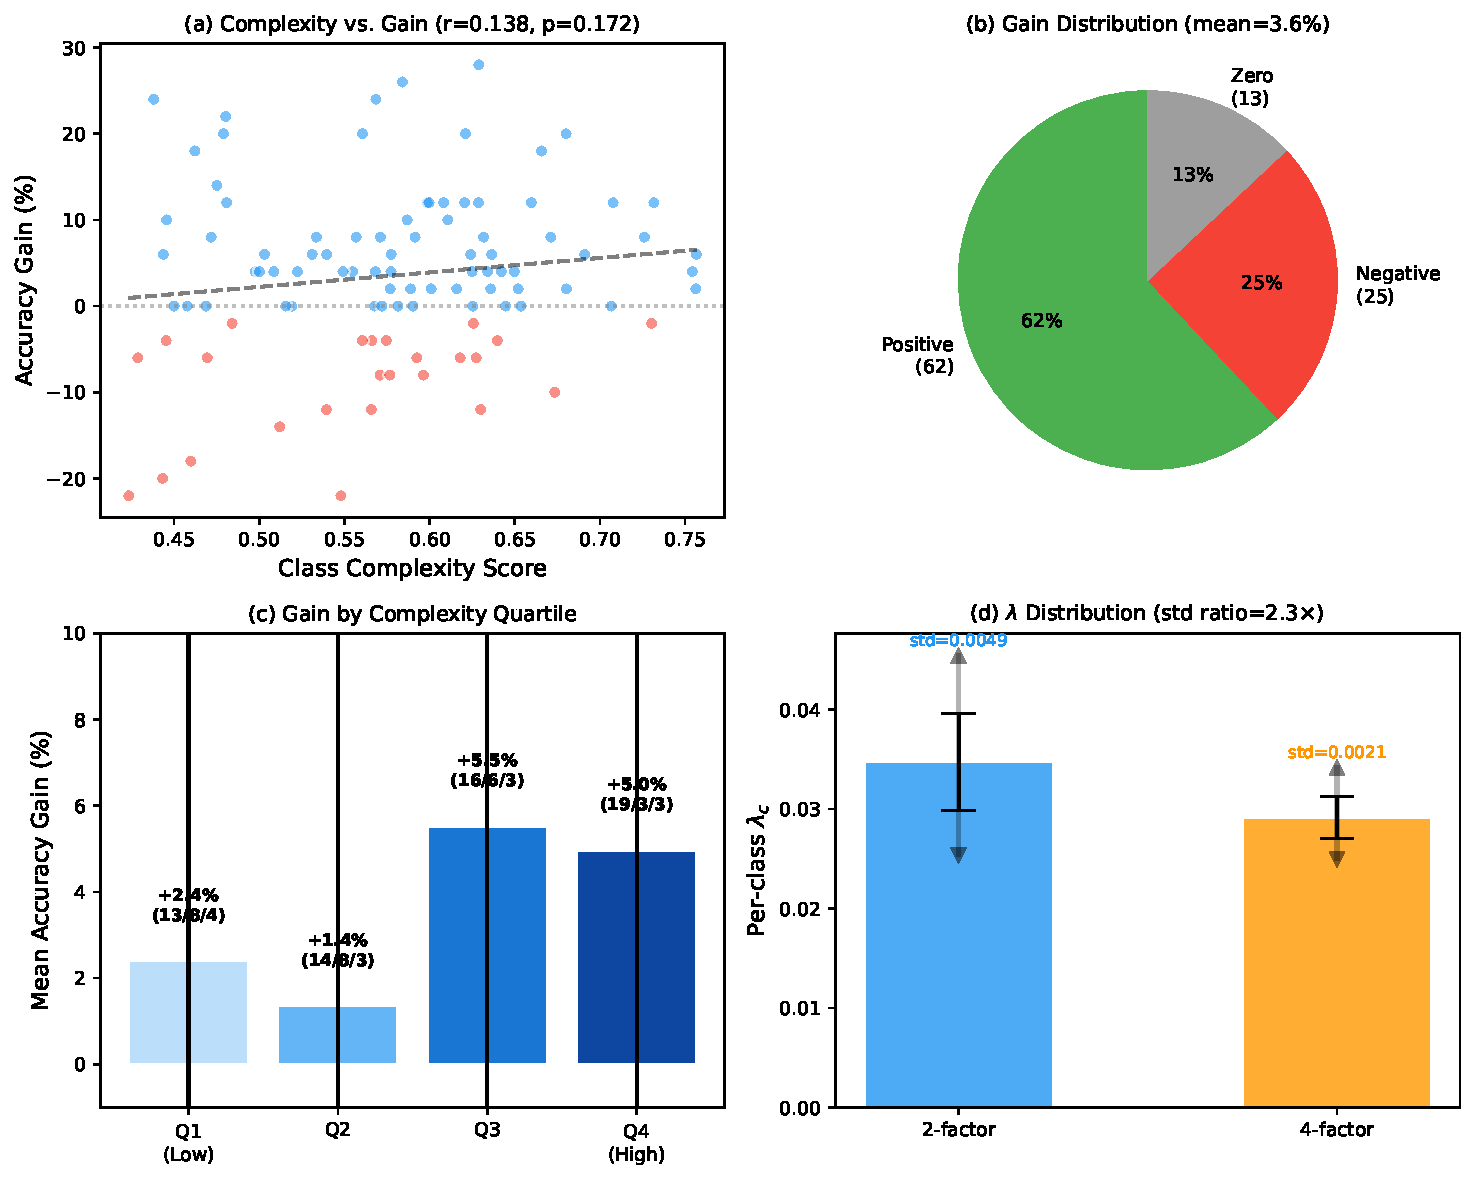
\includegraphics[width=\columnwidth]{figures/class_level_mechanism.pdf}
\caption{Class-level mechanism analysis. (a) Complexity vs.\ per-class gain scatter showing weak but positive correlation ($r{=}0.138$). (b) Distribution of per-class gains: $62\%$ positive, $25\%$ negative, $13\%$ zero. (c) Gain by complexity quartile: Q3 and Q4 (higher complexity) gain $2.8\times$ more than Q1 and Q2. (d) Per-class $\lambda_c$ distribution: the two-factor design (blue) produces $2.3\times$ wider variation than the four-factor design (orange).}
\label{fig:class-level-mechanism}
\end{figure}

\subsection{Sensitivity to Guidance Range}
\label{sec:sensitivity}

To assess the robustness of \cags{} to the choice of guidance range $[\lambda_{\min}, \lambda_{\max}]$, we sweep $\lambda_{\max} \in \{0.04, 0.06, 0.08, 0.10\}$ on the 100-class subset with IPC=10 and ConvNet-6 (\Cref{tab:sensitivity}). All configurations yield top-1 accuracy within a narrow band of $22.7$--$23.5\%$, well within the standard deviation of the main result ($\pm 0.47\%$). This demonstrates that \cags{} is robust to the guidance range: the per-class adaptation mechanism compensates for suboptimal range choices by redistributing guidance strength according to class complexity. Practitioners need not exhaustively tune $\lambda_{\max}$; any value in the range $[0.04, 0.10]$ produces comparable results. Notably, even the widest range $[0.0, 0.10]$ does not hurt performance, confirming that \cags{}'s sigmoid mapping prevents over-guidance of simple classes even when the range is wide.

\begin{table}[t]
\centering
\caption{Sensitivity to guidance range on ImageNet-100 (100-class) with ConvNet-6, IPC=10. All configurations yield comparable top-1 accuracy within $\sim$1\% of each other, demonstrating that \cags{} is robust to the choice of $\lambda_{\max}$. The $\lambda_{\max}=0.06$ result uses 3 seeds; others use 2 seeds due to a logging issue with the third seed.}
\label{tab:sensitivity}
\begin{tabular}{lccc}
\toprule
\textbf{$\lambda_{\max}$} & \textbf{Avg.\ $\lambda$} & \textbf{Top-1 (\%)} & \textbf{$\Delta$ vs.\ unguided} \\
\midrule
Unguided & 0.000 & $22.79 \pm 0.18$ & --- \\
\midrule
0.04 & $\sim$0.028 & $23.24$ & $+0.45$ \\
0.06 & $\sim$0.042 & $23.27 \pm 0.47$ & $+0.48$ \\
0.08 & $\sim$0.055 & $22.66$ & $-0.13$ \\
0.10 & $\sim$0.069 & $23.49$ & $+0.70$ \\
\bottomrule
\end{tabular}
\end{table}

\subsection{Computational Overhead}
\label{sec:compute-efficiency}

The \cags{} overhead consists of three one-time steps performed before dataset generation: (1) VAE feature extraction from real training images ($\sim$14 minutes for 131{,}689 images at $\sim$130 images/s on a single RTX 4090), (2) per-class KMeans clustering with silhouette-based $K$ selection ($\sim$8 minutes for 200 classes at $\sim$4.6 seconds per class), and (3) complexity score computation ($<1$ second). The total one-time overhead is approximately 22 minutes, after which the cached \texttt{ClassComplexityAnalyzer} object can be reused across all configurations---changing the complexity weights $(\alpha, \beta, \gamma, \delta)$ requires only a $<1$ second recomputation of the sigmoid mapping, with no need to re-extract features or re-run clustering. Dataset generation itself takes $\sim$16 minutes per configuration for 100 classes (IPC=10) or $\sim$33 minutes for 200 classes, dominated by the 50-step DiT denoising loop. Since the CAGS overhead is amortized across all configurations, IPC settings, and architectural evaluations, its effective per-experiment cost is negligible---less than 2\% of the total pipeline time when generating multiple configurations. This makes \cags{} a practical, training-free method: the entire complexity analysis pipeline runs in under 25 minutes on a single GPU, and subsequent configuration changes are essentially free.
